\chapter{الكيمياء الفراغية بتعمق}\label{ch:b1:stereochemistry-in-depth}

اسحق بضع بذور من الكراوية، ثم ورقة من النعناع: رائحتان
مختلفتان تمامًا. والمادة العطرية الرئيسية في كل منهما هي الكارفون، \ce{C10H14O}، بالذرات نفسها
مترابطة بالترتيب نفسه --- لكن الكارفونين صورتان مرآويتان
إحداهما للأخرى، كما اليد اليسرى صورة لليد اليمنى، ومستقبلات
الأنف، المبنية هي نفسها من جزيئات غير متناظرة مرآويًا، تميّز بينهما.
فالأدوية والمنكّهات وجزيئات الحياة كلها مبنية في الأبعاد
الثلاثة، والصيغة البنيوية التي تهمل البعد الثالث
تفوّت نصف القصة. يقدّم هذا الفصل أدوات رسم الجزيئات في
الفضاء، وتسمية كل ترتيب دون لبس، وتتبّع
الدورانات التي تجريها الجزيئات باستمرار، وقياس الخاصية
الفيزيائية الوحيدة التي تميّز بين الصورتين المرآويتين.

\begin{recall}
قدّم المجلد المدرسي (الصف الثاني عشر) الجزيئات \omterm{def:b1:stereochemistry-in-depth:stereocentre}{الكيرالية}، والكربون غير
المتناظر، \omterm{def:b1:stereochemistry-in-depth:enantiomers}{والمتماكبات المرآوية}، والمتماكبات $Z$/$E$ وتشكّلات الإيثان.
أما الترتيب الرباعي الأوجه للروابط الأربع حول الكربون ووصف
الروابط الأحادية والثنائية بالرابطتين $\sigma$/$\pi$ فمصدرهما
\cref{ch:b1:lewis-resonance-vsepr}.
\end{recall}

\begin{omfigure}
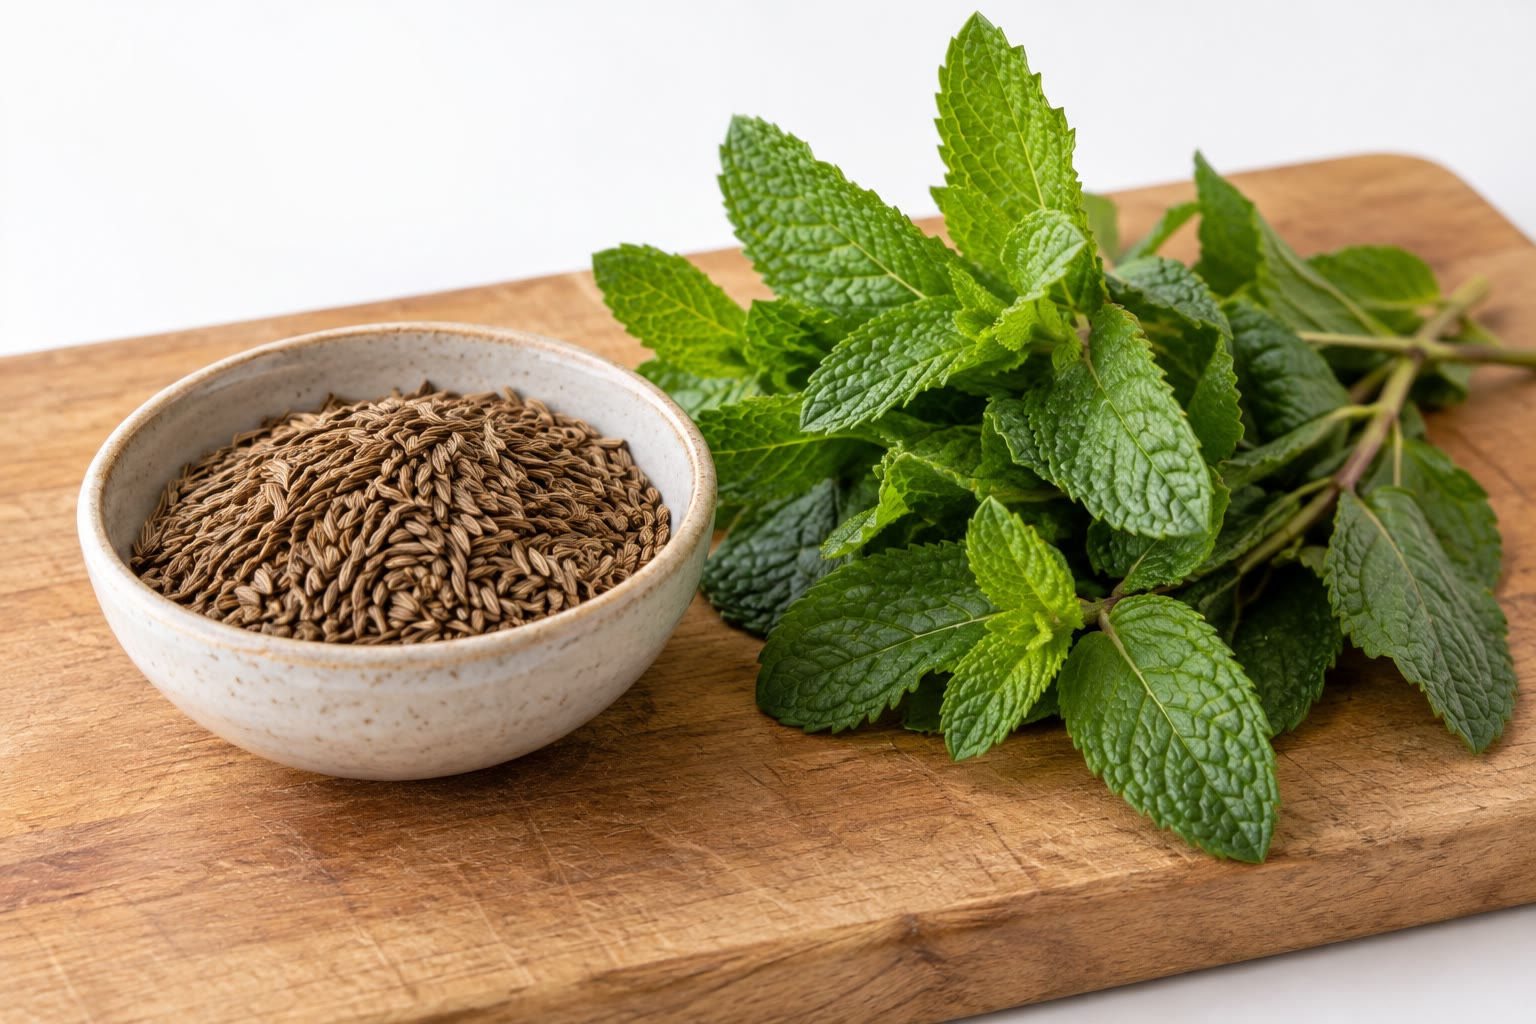
\includegraphics[width=0.55\linewidth]{images/book2/ai/b1-16-caraway-mint.jpg}

{\small بذور الكراوية وأوراق النعناع. تدين الكراوية برائحتها أساسًا
للكارفون-\cip{S}، والنعناع لصورته المرآوية، الكارفون-\cip{R}.}
\end{omfigure}

\section{المتماكبات وطرائق التمثيل}

\begin{definition}[البنية، الترتيب الفراغي، التشكّل]\label{def:b1:stereochemistry-in-depth:isomers}
المركبان اللذان لهما الصيغة نفسها وترتبط ذراتهما بترتيب
مختلف \emph{متماكبات بنيوية}\index{متماكبات بنيوية}.
والمركبات التي لها البنية نفسها ولا تختلف ذراتها إلا في
ترتيبها في الفضاء \emph{متماكبات فراغية}\index{متماكبات فراغية}.
والترتيب الذي لا يمكن تغييره إلا بكسر روابط هو
\emph{الترتيب الفراغي}\index{ترتيب فراغي} للمتماكب الفراغي؛ أما
الترتيب الناتج عن الدوران حول روابط أحادية، دون كسر أي منها،
فهو \emph{تشكّل}\index{تشكّل}.
\end{definition}

في درجة حرارة الغرفة تجري الدورانات حول الروابط الأحادية مليارات
المرات في الثانية: فتتحول التشكّلات بعضها إلى بعض ولا يمكن عزلها، بينما
الترتيبات الفراغية مستقرة وتعطي مركبات متمايزة.

\begin{definition}[طرائق التمثيل]\label{def:b1:stereochemistry-in-depth:representations}
في \emph{تمثيل كرام}\index{تمثيل كرام} تُرسم رابطتان
في مستوي الصفحة، ويتجه الإسفين الممتلئ نحو
القارئ والإسفين المخطط بعيدًا عنه. و\emph{إسقاط نيومان}\index{إسقاط نيومان}
ينظر إلى الجزيء على امتداد رابطة C--C واحدة: فالكربون الأمامي
نقطة تلتقي فيها روابطه الثلاث الأخرى، والكربون الخلفي دائرة تنبثق
روابطه من محيطها. وفي \emph{إسقاط فيشر}\index{إسقاط فيشر}
تكون السلسلة الكربونية رأسية، وتتجه الروابط الأفقية نحو
القارئ والروابط الرأسية بعيدًا عنه؛ وكل تقاطع كربون فراغي المركز.
\end{definition}

\begin{omfigure}
\begin{tikzpicture}[font=\small]
  % staggered and eclipsed ethane, Newman
  \pic (s) at (0,0) {omnewman={90}{30}};
  \foreach \k in {1,2,3} { \node at (s-f\k) {H}; \node at (s-b\k) {H}; }
  \node at (0,-1.9) {متخالف};
  \pic (e) at (3.6,0) {omnewman={90}{108}};
  \foreach \k in {1,2,3} { \node at (e-f\k) {H}; }
  \foreach \k in {1,2,3} { \node[font=\scriptsize, black!60] at ($(e-b\k)!-0.12!(e-c)$) {H}; }
  \node at (3.6,-1.9) {متطابق};
  % Fischer projection of (R)-lactic acid
  \begin{scope}[xshift=7.6cm]
    \draw[thick] (-0.9,0) -- (0.9,0) (0,-0.9) -- (0,0.9);
    \node[above] at (0,0.9) {\ce{COOH}};
    \node[below] at (0,-0.9) {\ce{CH3}};
    \node[left] at (-0.9,0) {H};
    \node[right] at (0.9,0) {OH};
    \node at (0,-1.9) {فيشر};
  \end{scope}
  % Cram of the same
  \begin{scope}[xshift=11.0cm]
    \node at (0,0) {\chemfig{C(-[2]COOH)(-[:210]H_3C)(<:[:-12]OH)(<[:-55]H)}};
    \node at (0,-1.9) {كرام};
  \end{scope}
\end{tikzpicture}

{\small يسارًا: إسقاطا نيومان للإيثان على امتداد رابطته C--C، المتخالف
(الروابط الخلفية بين الأمامية) والمتطابق (الروابط الخلفية مختبئة
خلف الأمامية، مرسومة مزاحة قليلًا). يمينًا: الجزيء نفسه،
حمض اللبن-\cip{R}، في \omterm{def:b1:stereochemistry-in-depth:representations}{إسقاط فيشر} وفي \omterm{def:b1:stereochemistry-in-depth:representations}{تمثيل كرام}
(روابط صليب فيشر الرأسية تتجه بعيدًا عن القارئ،
والأفقية نحوه).}
\end{omfigure}

\begin{method}[من كرام إلى نيومان]\label{met:b1:stereochemistry-in-depth:newman-from-cram}
\begin{enumerate}
  \item اختر الرابطة التي يُنظر على امتدادها والطرف الأقرب إلى العين.
  \item ارسم روابط الكربون الأمامي الثلاث انطلاقًا من المركز،
        محافظًا على ترتيبها (في اتجاه عقارب الساعة أو عكسه) كما تراه
        العين.
  \item ارسم روابط الكربون الخلفي انطلاقًا من الدائرة، بترتيبها كما
        يُرى من الجهة نفسها.
  \item تحقق: تدوير الكربون الخلفي بزاوية $60^\circ$ ينقل من
        المتخالف إلى المتطابق؛ وبزاوية $120^\circ$، من \omterm{def:b1:stereochemistry-in-depth:conformations}{تشكّل متخالف}
        إلى التالي.
\end{enumerate}
\end{method}

\section{الترتيب الفراغي: قواعد CIP}

\begin{definition}[قواعد CIP، الواصفات]\label{def:b1:stereochemistry-in-depth:cip}
\emph{قواعد CIP}\index{قواعد CIP} (كان--إنغولد--بريلوغ) ترتّب
المتبادلات الأربعة \omterm{def:b1:stereochemistry-in-depth:stereocentre}{لمركز فراغي}: العدد الذري الأعلى أولًا؛ وعند
التساوي، تُقارن مجموعات الذرات المرتبطة بعدها، وهكذا إلى الخارج؛
وتُعدّ الرابطة الثنائية رابطتين أحاديتين إلى ذرات مكرَّرة. ومع
اتجاه المتبادل الأدنى رتبةً بعيدًا عن العين، يعرّف دوران التسلسل
$1 \to 2 \to 3$ في اتجاه عقارب الساعة الواصف \cip{R}،
وعكسها الواصف \cip{S}. ومن أجل رابطة ثنائية على كل من كربونيها متبادلان،
يعني \cip{Z} أن المتبادلين الأعلى رتبةً في الجهة نفسها
و\cip{E} أنهما في جهتين متعاكستين.
\end{definition}

\begin{method}[تعيين الواصف \texorpdfstring{\babelsublr{\cip{R}}}{(R)} أو \texorpdfstring{\babelsublr{\cip{S}}}{(S)} \omterm{def:b1:stereochemistry-in-depth:stereocentre}{لمركز فراغي}]\label{met:b1:stereochemistry-in-depth:cip}
\begin{enumerate}
  \item رتّب المتبادلات الأربعة وفق \omterm{def:b1:stereochemistry-in-depth:cip}{قواعد CIP}.
  \item إذا كان الأدنى رتبةً متجهًا بعيدًا عنك (إسفين مخطط، أو
        رابطة رأسية في \omterm{def:b1:stereochemistry-in-depth:representations}{إسقاط فيشر})، فاقرأ اتجاه دوران
        $1 \to 2 \to 3$ مباشرة.
  \item إذا كان متجهًا نحوك (إسفين ممتلئ، أو رابطة فيشر أفقية)،
        فاقرأ الدوران واعكس الواصف.
  \item تبادل أي متبادلين يعكس الواصف: وهذا
        تحقق سريع.
\end{enumerate}
في حمض اللبن، $\ce{OH} > \ce{COOH} > \ce{CH3} > \ce{H}$ (O؛ ثم \babelsublr{C(O,O,O)}
يتقدم على \babelsublr{C(H,H,H)}). وفي \omterm{def:b1:stereochemistry-in-depth:representations}{إسقاط فيشر} أعلاه، H أفقية
(نحونا) و$\ce{OH} \to \ce{COOH} \to \ce{CH3}$ تدور عكس عقارب الساعة:
وبعد العكس، يكون المركز \cip{R}.
\end{method}

\section{الكيرالية ونتائجها}

\begin{definition}[المركز الفراغي، الكيرالية]\label{def:b1:stereochemistry-in-depth:stereocentre}
يكون الجسم \emph{كيراليًا}\index{كيرالي} إذا لم يمكن تطبيقه على
صورته المرآوية، و\emph{لاكيراليًا}\index{لاكيرالي} في الحالة الأخرى؛ والخاصية هي
\emph{الكيرالية}\index{كيرالية}. و\emph{المركز
الفراغي}\index{مركز فراغي} ذرة يعطي تبادل متبادلين عندها
\omterm{def:b1:stereochemistry-in-depth:isomers}{متماكبًا فراغيًا}؛ والكربون الرباعي الأوجه ذو المتبادلات الأربعة
المختلفة مركز من هذا النوع.
\end{definition}

الجزيء الذي له مستوي تناظر أو مركز تناظر \omterm{def:b1:stereochemistry-in-depth:stereocentre}{لاكيرالي}؛
والجزيء الذي ليس له أي منهما \omterm{def:b1:stereochemistry-in-depth:stereocentre}{كيرالي} عمليًا. أما المعيار الدقيق، بلغة
عمليات التناظر، فيعطيه مجلد السنة الثالثة.

\begin{definition}[المتماكبات المرآوية، المتماكبات اللامرآوية، مركب ميزو، الخليط الراسيمي]\label{def:b1:stereochemistry-in-depth:enantiomers}
\omterm{def:b1:stereochemistry-in-depth:isomers}{المتماكبان الفراغيان} اللذان كل منهما صورة مرآوية للآخر
\emph{متماكبات مرآوية}\index{متماكبات مرآوية}؛ \omterm{def:b1:stereochemistry-in-depth:isomers}{والمتماكبات الفراغية} التي ليست كذلك
\emph{متماكبات لامرآوية}\index{متماكبات لامرآوية}. و\emph{مركب
الميزو}\index{مركب ميزو} له مراكز فراغية لكنه \omterm{def:b1:stereochemistry-in-depth:stereocentre}{لاكيرالي}.
والخليط المتساوي المولات من متماكبين مرآويين \emph{خليط
راسيمي}\index{خليط راسيمي}.
\end{definition}

\begin{proposition}[عدد المتماكبات الفراغية]\label{prop:b1:stereochemistry-in-depth:max-stereoisomers}
للجزيء ذي $n$ مركزًا فراغيًا (ولا وحدة فراغية أخرى) على الأكثر
$2^n$ \omterm{def:b1:stereochemistry-in-depth:isomers}{متماكبًا فراغيًا}، في $2^{n-1}$ زوجًا على الأكثر من
\omterm{def:b1:stereochemistry-in-depth:enantiomers}{المتماكبات المرآوية}؛ وأشكال الميزو تقلل هذا العدد.
\end{proposition}

\begin{proof}
كل مركز إما \cip{R} وإما \cip{S} باستقلال: $2^n$ تركيبة.
والصورة المرآوية تغيّر كل واصف، فتتزاوج التركيبات في
\omterm{def:b1:stereochemistry-in-depth:enantiomers}{متماكبات مرآوية}، $2^{n-1}$ زوجًا. وإذا كانت تركيبة ما صورة مرآوية لنفسها
بعد تدوير الجزيء (شكل ميزو)، اندمج زوجها في
مركب واحد.
\end{proof}

لحمض الطرطريك، \ce{HOOC-CH(OH)-CH(OH)-COOH}، مركزان متكافئان:
\cip{R,R} و\cip{S,S} \omterm{def:b1:stereochemistry-in-depth:enantiomers}{متماكبان مرآويان}، بينما يملك المتماكب \cip{R,S} مستوي مرآة
بين الكربونين فهو ميزو: ثلاثة \omterm{def:b1:stereochemistry-in-depth:isomers}{متماكبات فراغية}، لا أربعة.

\begin{proposition}[خواص المتماكبات المرآوية]\label{prop:b1:stereochemistry-in-depth:enantiomer-properties}
\omterm{def:b1:stereochemistry-in-depth:enantiomers}{للمتماكبين المرآويين} درجتا الانصهار والغليان نفساهما، \omterm{def:b1:precipitation:solubility}{والذوبانية} نفسها
في المذيبات اللاكيرالية، والأطياف نفسها، والتفاعلية نفسها تجاه الكواشف اللاكيرالية؛
ويختلفان في تأثيرهما في الضوء المستقطب وفي تآثراتهما
مع الجزيئات \omterm{def:b1:stereochemistry-in-depth:stereocentre}{الكيرالية} الأخرى. أما \omterm{def:b1:stereochemistry-in-depth:enantiomers}{المتماكبات اللامرآوية} فتختلف في كل
خواصها.
\end{proposition}

\begin{proof}
كل خاصية لا تتعلق إلا بالمسافات والزوايا داخل
الجزيء، أو بينه وبين شركاء لاكيراليين، هي نفسها للجسم
وصورته المرآوية، لأن الانعكاس يحفظ المسافات
والزوايا. أما الشريك \omterm{def:b1:stereochemistry-in-depth:stereocentre}{الكيرالي} (مستقبِل، أو كاشف \omterm{def:b1:stereochemistry-in-depth:stereocentre}{كيرالي}، أو المسار الحلزوني
للضوء المستقطب الموصوف أدناه) فيكوّن أزواجًا لامرآوية فيما بينها،
لم تعد صورًا مرآوية، فتختلف إذن. ولا يربط بين \omterm{def:b1:stereochemistry-in-depth:enantiomers}{المتماكبات اللامرآوية}
أي انعكاس: فمسافاتها الداخلية مختلفة.
\end{proof}

\begin{omfigure}
\begin{tikzpicture}[font=\small, line join=round]
  \foreach \dx/\kind/\lab in {0/1/{\foreignlanguage{arabic}{الكارفون-\babelsublr{\cip{R}}، النعناع}}, 5.2/0/{\foreignlanguage{arabic}{الكارفون-\babelsublr{\cip{S}}، الكراوية}}} {
  \begin{scope}[xshift=\dx cm]
    \coordinate (c1) at (0,1); \coordinate (c2) at (0.87,0.5);
    \coordinate (c3) at (0.87,-0.5); \coordinate (c4) at (0,-1);
    \coordinate (c5) at (-0.87,-0.5); \coordinate (c6) at (-0.87,0.5);
    \draw[thick] (c1) -- (c2) -- (c3) -- (c4) -- (c5) -- (c6) -- cycle;
    \draw[thick] ($(c2)!0.15!(c3)+(-0.12,0)$) -- ($(c3)!0.15!(c2)+(-0.12,0)$);
    \draw[thick] (c1) -- ++(0,0.7) node[above] {O};
    \draw[thick] ($(c1)+(0.1,0)$) -- ++(0,0.62);
    \draw[thick] (c2) -- ++(0.75,0.43) node[right] {\ce{CH3}};
    \coordinate (q) at ($(c5)+(-0.75,-0.43)$);
    \ifnum\kind=1
      \fill (c5) -- ($(q)+(0.06,-0.1)$) -- ($(q)+(-0.06,0.1)$) -- cycle;
    \else
      \foreach \t in {0.15,0.3,0.45,0.6,0.75,0.9}
        \draw ($(c5)!\t!(q)+(\t*0.06,-\t*0.1)$) -- ($(c5)!\t!(q)+(-\t*0.06,\t*0.1)$);
    \fi
    \draw[thick] (q) -- ++(-0.6,0.5) node[above] {\ce{CH2}};
    \draw[thick] ($(q)+(0.08,0.06)$) -- ++(-0.6,0.5);
    \draw[thick] (q) -- ++(0,-0.75) node[below] {\ce{CH3}};
    \node[font=\scriptsize] at ($(c5)+(0.35,0.12)$) {5};
    \node at (0,-2.85) {\lab};
  \end{scope}}
\end{tikzpicture}

{\small الكارفونان مرسومين على الهيكل نفسه: مجموعة الإيزوبروبينيل
على C5 تتجه نحو القارئ (إسفين ممتلئ) في أحدهما وبعيدًا عن
القارئ (إسفين مخطط) في الآخر، وهيدروجين C5 (غير المرسوم) في
الجهة المقابلة. وهما صورتان مرآويتان إحداهما للأخرى: \omterm{def:b1:stereochemistry-in-depth:enantiomers}{متماكبان مرآويان}
(\cref{exo:b1:stereochemistry-in-depth:4}).}
\end{omfigure}

\begin{history}[الكربون الرباعي الأوجه]
\begin{minipage}[t]{0.2\linewidth}\vspace{0pt}
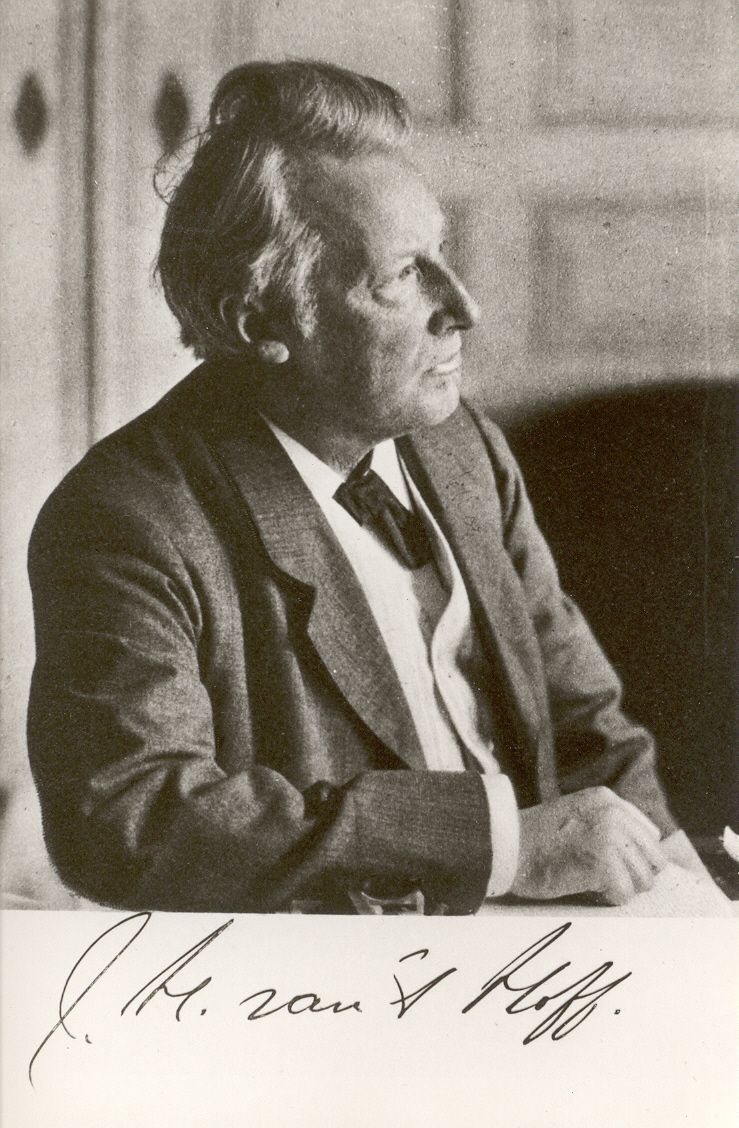
\includegraphics[width=\linewidth]{images/book2/van-t-hoff.jpg}
\end{minipage}\hfill
\begin{minipage}[t]{0.76\linewidth}\vspace{0pt}
اقترح ياكوبوس هنريكوس فانت هوف، وهو كيميائي شاب، أن روابط ذرة الكربون
الأربع تتجه نحو رؤوس رباعي أوجه. فيوجد الكربون
ذو المتبادلات الأربعة المختلفة عندئذ على هيئة ترتيبين كل منهما صورة مرآوية
للآخر، وهذا ما فسّر لماذا تأتي بعض المركبات في شكلين لا
يختلفان إلا في طريقة تدويرهما للضوء المستقطب. والفكرة هي
نقطة انطلاق كل رسم في هذا الفصل.
(صورة نُشرت سنة 1911، ملكية عامة، ويكيميديا كومنز.)
\end{minipage}
\end{history}

\section{التشكّلات}

\begin{definition}[زاوية الالتواء والتشكّلات]\label{def:b1:stereochemistry-in-depth:conformations}
من أجل أربع ذرات A--B--C--D، تكون \emph{زاوية الالتواء}\index{زاوية الالتواء}
$\theta$ حول B--C هي الزاوية بين المستويين ABC وBCD، وتُقرأ على
\omterm{def:b1:stereochemistry-in-depth:representations}{إسقاط نيومان} على امتداد B--C. ويكون \omterm{def:b1:stereochemistry-in-depth:isomers}{التشكّل} \emph{تشكّلًا
متطابقًا}\index{تشكّل متطابق} حين تتراصف روابط الكربونين الأمامي
والخلفي في الإسقاط، و\emph{تشكّلًا
متخالفًا}\index{تشكّل متخالف} حين تتناوب. وفي
البوتان، منظورًا إليه على امتداد C2--C3، يكون \omterm{def:b1:stereochemistry-in-depth:isomers}{التشكّل} المتخالف الذي فيه
مجموعتا الميثيل على $180^\circ$ هو \emph{التشكّل المضاد}\index{تشكّل مضاد}،
والتشكّلان اللذان فيهما على $\pm 60^\circ$ هما \emph{التشكّلان
المنحرفان}\index{تشكّل منحرف}. وفي الهكسان الحلقي، تكون
الحلقة المجعّدة الخالية من الإجهاد هي \emph{الكرسي}\index{كرسي}؛ ويحمل كل كربون
رابطة \emph{محورية}\index{محوري} واحدة، موازية لمحور
الحلقة، ورابطة \emph{استوائية}\index{استوائي} واحدة، تقع تقريبًا في
المستوي المتوسط للحلقة. و\emph{انقلاب الحلقة}\index{انقلاب الحلقة} يحوّل
كرسيًا إلى الآخر، فتصير كل رابطة محورية استوائية
والعكس.
\end{definition}

\begin{omfigure}
\begin{tikzpicture}
\begin{axis}[
  width=0.82\linewidth, height=5.8cm, xmin=0, xmax=360, ymin=0, ymax=21,
  legend style={font=\scriptsize, draw=none, at={(0.5,0.62)}, anchor=center},
  axis x line=bottom, axis y line=left, xlabel={\foreignlanguage{arabic}{زاوية الالتواء $\theta$ بالدرجات}},
  ylabel={\foreignlanguage{arabic}{الطاقة \babelsublr{(kJ/mol)}}}, xtick={0,60,120,180,240,300,360},
  tick label style={font=\small}, label style={font=\small}]
\addplot[omDef, very thick] table[x=theta, y=butane] {figdata/out/bachelor-1-butane-torsion.dat};
\addplot[omProp, thick, dashed] table[x=theta, y=ethane] {figdata/out/bachelor-1-butane-torsion.dat};
\node[font=\scriptsize, anchor=south west] at (axis cs:0,18.4) {متزامن};
\node[font=\scriptsize, anchor=south] at (axis cs:62,18.4) {منحرف};
\node[font=\scriptsize, anchor=south] at (axis cs:120,18.4) {متطابق};
\node[font=\scriptsize, anchor=south] at (axis cs:180,18.4) {مضاد};
\node[font=\scriptsize, anchor=south] at (axis cs:240,18.4) {متطابق};
\node[font=\scriptsize, anchor=south] at (axis cs:298,18.4) {منحرف};
\node[font=\scriptsize, anchor=south east] at (axis cs:360,18.4) {متزامن};
\legend{{البوتان}, {الإيثان}}
\end{axis}
\end{tikzpicture}

{\small طاقة الالتواء للبوتان حول رابطته المركزية (الخط المتصل؛ $\theta
= 0$ حين تتطابق مجموعتا الميثيل) وللإيثان (الخط المتقطع)،
محسوبة من كمونات التواء تجريبية. الإيثان: الحاجز
\qty{12.2}{kJ/mol}. البوتان: المضاد هو الأكثر استقرارًا؛ والمنحرف أعلى منه بمقدار \qty{2.8}{kJ/mol}،
عند $\theta = 62^\circ$؛ والحاجزان \qty{15.2}{kJ/mol} (ميثيل
يطابق هيدروجينًا) و\qty{16.5}{kJ/mol} (ميثيل يطابق ميثيلًا).}
% ledger: rot:ethane-V3, rot:butane-V1, rot:butane-V2, rot:butane-V3, rot:butane-V4, rot:butane-V5, rot:butane-V6 (curves in figdata/bachelor-1/butane-torsion.py)
\end{omfigure}

الحواجز صغيرة مقارنةً بالطاقة الحرارية المتاحة في
الاصطدامات ($RT = \qty{2.5}{kJ/mol}$ في درجة حرارة الغرفة، وأكثر بكثير في
ذيل التوزيع، \cref{ch:b1:elementary-steps}): فالدوران
سريع، والبوتان خليط من جزيئات مضادة ومنحرفة لا يمكن
فصلها.

\begin{method}[رسم الكرسي]\label{met:b1:stereochemistry-in-depth:draw-chair}
\begin{enumerate}
  \item ارسم خطين متوازيين مائلين قليلًا نحو الأسفل إلى اليمين،
        مزاحين؛ وصل طرفيهما بحرف V في اليسار وبحرف V مقلوب في
        اليمين لتغلق الحلقة السداسية.
  \item الروابط \omterm{def:b1:stereochemistry-in-depth:conformations}{المحورية} رأسية: إلى الأعلى على الكربونات المتجهة إلى الأعلى، وإلى الأسفل على
        المتجهة إلى الأسفل، بالتناوب حول الحلقة.
  \item الروابط \omterm{def:b1:stereochemistry-in-depth:conformations}{الاستوائية} موازية لروابط الحلقة التي تليها بعد واحدة،
        وتتجه نحو الخارج.
  \item لقلب الحلقة، ارسم \omterm{def:b1:stereochemistry-in-depth:conformations}{الكرسي} الآخر؛ فالمتبادل \omterm{def:b1:stereochemistry-in-depth:conformations}{المحوري} في أحدهما
        \omterm{def:b1:stereochemistry-in-depth:conformations}{استوائي} في الآخر.
\end{enumerate}
\end{method}

\begin{omfigure}
\begin{tikzpicture}[font=\small]
  \pic (a) at (0,0) {omchair};
  \foreach \k in {1,2,3,4,5,6} \draw[omProp, thick] (a-c\k) -- (a-a\k);
  \foreach \k in {1,2,3,4,5,6} \draw[omDef, thick] (a-c\k) -- (a-e\k);
  \node[omProp, anchor=south] at (a-a3) {محورية};
  \node[omDef, anchor=north] at (a-e5) {استوائية};
  \begin{scope}[xshift=4.9cm]
    \pic (b) at (0,0) {omchair};
    \draw[thick] (b-c1) -- (b-e1) node[right] {\ce{CH3}};
    \draw[thick] (b-c1) -- (b-a1) node[above] {H};
    \node at (0,-1.5) {\foreignlanguage{arabic}{\ce{CH3} استوائي}};
  \end{scope}
  \draw[<->, thick] (8.1,0) -- (8.8,0) node[midway, above] {انقلاب};
  \begin{scope}[xshift=10.45cm]
    \pic (c) at (0,0) {omchairflip};
    \draw[thick] (c-c4) -- (c-a4) node[below] {\ce{CH3}};
    \draw[thick] (c-c4) -- (c-e4) node[right] {H};
    \node at (0,-1.5) {\foreignlanguage{arabic}{\ce{CH3} محوري}};
  \end{scope}
\end{tikzpicture}

{\small يسارًا: \omterm{def:b1:stereochemistry-in-depth:conformations}{كرسي} الهكسان الحلقي بروابطه \omterm{def:b1:stereochemistry-in-depth:conformations}{المحورية} الست (بالبرتقالي،
إلى الأعلى وإلى الأسفل بالتناوب) وروابطه \omterm{def:b1:stereochemistry-in-depth:conformations}{الاستوائية} الست (بالأزرق). يمينًا: الكرسيان
لميثيل الهكسان الحلقي، اللذان يتحول أحدهما إلى الآخر \omterm{def:b1:stereochemistry-in-depth:conformations}{بانقلاب الحلقة}؛ ومجموعة
الميثيل \omterm{def:b1:stereochemistry-in-depth:conformations}{استوائية} في أحدهما، \omterm{def:b1:stereochemistry-in-depth:conformations}{ومحورية} في الآخر.}
\end{omfigure}

\begin{proposition}[المتبادلات الاستوائية مفضَّلة]\label{prop:b1:stereochemistry-in-depth:chair-substituent}
في الهكسان الحلقي الأحادي الاستبدال يكون \omterm{def:b1:stereochemistry-in-depth:conformations}{الكرسي} الذي فيه المتبادل
\omterm{def:b1:stereochemistry-in-depth:conformations}{استوائي} هو الأكثر استقرارًا. وفي مجموعة الميثيل، يضيف الموضع \omterm{def:b1:stereochemistry-in-depth:conformations}{المحوري}
تآثرين منحرفين مع كربونات الحلقة، قيمة كل منهما قيمة تآثر البوتان
(\qtyrange{2.8}{2.9}{kJ/mol})، أي نحو \qty{5.7}{kJ/mol} إجمالًا: وهذا تقدير
لفرق الطاقة.
\end{proposition}

\begin{proof}
منظورًا على امتداد الرابطة C1--C2، يكون الميثيل \omterm{def:b1:stereochemistry-in-depth:conformations}{المحوري} على C1 منحرفًا بالنسبة إلى C3
من الحلقة؛ ومنظورًا على امتداد C1--C6، منحرفًا بالنسبة إلى C5: أي تآثران منحرفان من
نوع البوتان، يُريان أيضًا ازدحامًا للميثيل مع
الهيدروجينات \omterm{def:b1:stereochemistry-in-depth:conformations}{المحورية} على C3 وC5 (التآثرات 1،3-ثنائية المحور). أما
الميثيل \omterm{def:b1:stereochemistry-in-depth:conformations}{الاستوائي} فمضاد بالنسبة إلى C3 وC5. وكل تآثر منحرف يكلّف
ما يكلّفه في البوتان، \qty{2.8}{kJ/mol} في كمون الالتواء في
الشكل.
\end{proof}

مع $\Delta E = \qty{5.7}{kJ/mol}$، تكون نسبة الكراسي \omterm{def:b1:stereochemistry-in-depth:conformations}{الاستوائية} إلى \omterm{def:b1:stereochemistry-in-depth:conformations}{المحورية}
عند \qty{25}{\celsius} هي $\exp(\Delta E/RT) = 10$: أي نحو
\qty{91}{\percent} \omterm{def:b1:stereochemistry-in-depth:conformations}{استوائية} (\cref{exo:b1:stereochemistry-in-depth:9}).
والمجموعات الكبيرة، مثل ثالثي البوتيل، تثبّت الحلقة في \omterm{def:b1:stereochemistry-in-depth:conformations}{الكرسي} الذي تكون فيه
\omterm{def:b1:stereochemistry-in-depth:conformations}{استوائية}.

\section{النشاط الضوئي}

\begin{definition}[النشاط الضوئي، الدوران النوعي]\label{def:b1:stereochemistry-in-depth:optical-activity}
تُظهر مادة \emph{نشاطًا ضوئيًا}\index{نشاط ضوئي} إذا كانت
تدوّر مستوي استقطاب الضوء المستقطب خطيًا الذي يجتازها.
وكما يراها مراقب يواجه الضوء، فإن المادة
\emph{اليمينية الدوران}\index{يميني الدوران}، وتُكتب $(+)$،
تدوّره في اتجاه عقارب الساعة، و\emph{اليسارية الدوران}\index{يساري الدوران}،
$(-)$، عكسها. و\emph{الدوران النوعي}\index{دوران نوعي}
هو $[\alpha] = \alpha/(\ell c)$، حيث $\alpha$ الزاوية
المقيسة بالدرجات، و$\ell$ طول المسار بالديسيمتر و$c$ التركيز
الكتلي بالوحدة \unit{g/mL}؛ وهو يتعلق بطول الموجة (وهو عادةً
خط الصوديوم الأصفر)، وبدرجة الحرارة وبالمذيب.
\end{definition}

\begin{omfigure}
\begin{tikzpicture}[font=\small, >={Stealth}]
  \fill[yellow!70!orange] (0,0) circle (0.25);
  \node[below] at (0,-0.45) {المصباح};
  \draw[thick] (1.3,-0.7) rectangle (1.45,0.7); \node[below] at (1.37,-0.75) {المستقطِب};
  \draw[omDef!20, fill=omDef!10] (2.4,-0.45) rectangle (5.6,0.45);
  \node at (4.0,0) {\foreignlanguage{arabic}{العيّنة، طولها $\ell$}};
  \draw[thick] (6.5,-0.7) rectangle (6.65,0.7); \node[below] at (6.57,-0.75) {المحلِّل};
  \draw (7.6,0) circle (0.3); \node[below] at (7.6,-0.45) {العين};
  \draw[->, orange!80!black] (0.3,0) -- (1.25,0);
  \draw[->, orange!80!black] (1.5,0) -- (2.35,0);
  \draw[->, orange!80!black] (5.65,0) -- (6.45,0);
  % polarisation planes
  \draw[thick, omThm] (1.9,-0.35) -- (1.9,0.35);
  \draw[thick, omThm] (6.05,-0.33) -- ++(70:0.0) -- (5.93,0.33);
  \draw[->, omThm] (5.75,0.55) arc[start angle=100, end angle=70, radius=0.6];
  \node[omThm, above] at (6.1,0.75) {$\alpha$};
\end{tikzpicture}

{\small مقياس الاستقطاب. يمرر المستقطِب الضوء المهتز في مستوٍ
واحد؛ وتدوّر العيّنة \omterm{def:b1:stereochemistry-in-depth:stereocentre}{الكيرالية} ذلك المستوي بزاوية $\alpha$؛ ثم يُدار المحلِّل
حتى ينطفئ الضوء من جديد، وهذا يقيس $\alpha$.}
\end{omfigure}

\begin{proposition}[قانون بيو]\label{prop:b1:stereochemistry-in-depth:biot}
في محلول مخفف لعدة مذابات نشطة ضوئيًا، تكون زاوية
الدوران جمعية، $\alpha = \ell\sum_i [\alpha]_i c_i$ (\emph{قانون
بيو}\index{قانون بيو}). وللمتماكبين المرآويين دورانان نوعيان
متعاكسان؛ \omterm{def:b1:stereochemistry-in-depth:enantiomers}{والخليط الراسيمي} لا يدوّر الضوء.
\end{proposition}

\begin{proof}
يسهم كل مذاب باستقلال في المحلول المخفف، بالتناسب
مع عدد الجزيئات التي يجتازها الضوء، أي مع $\ell c_i$؛ وهذا هو
المضمون التجريبي للقانون. والانعكاس يحوّل اتجاه عقارب الساعة إلى
عكسه: فالجزيء الذي هو صورة مرآوية يدوّر المستوي بالزاوية
المعاكسة، وفي \omterm{def:b1:stereochemistry-in-depth:enantiomers}{الخليط الراسيمي} يلغي الإسهامان أحدهما الآخر.
\end{proof}

ومن أجل خليط من \omterm{def:b1:stereochemistry-in-depth:enantiomers}{متماكبين مرآويين} تركيزه الكلي $c$، يعطي الكسر
$x$ من الشكل $(-)$ الزاوية $\alpha = \ell c[\alpha]_{(-)}(x - (1 - x)) =
\ell c[\alpha]_{(-)}(2x - 1)$: فقياس $\alpha$ يعطي التركيب.
ولا يرتبط الدوران الضوئي بأي طريقة بسيطة بالواصف: فالمركب
\cip{R} قد يكون $(+)$ أو $(-)$؛ والكارفون-\cip{R} في النعناع
\omterm{def:b1:stereochemistry-in-depth:optical-activity}{يساري الدوران}.

\section{تمارين}

\begin{exercise}[$\star$]\label{exo:b1:stereochemistry-in-depth:1}
صنّف كل زوج إلى \omterm{def:b1:stereochemistry-in-depth:isomers}{متماكبين بنيويين}، أو مرآويين، أو لامرآويين،
أو تشكّلين لمركب واحد: البوتان-1-أول والبوتان-2-أول؛
البوتان-2-أول-\cip{R} و-\cip{S}؛ البوت-2-ين-\cip{Z} و-\cip{E}؛ التشكّلان المضاد
والمنحرف للبوتان؛ حمض الطرطريك-\cip{R,R} و-\cip{R,S}.
\end{exercise}

\begin{exercise}[$\star$]\label{exo:b1:stereochemistry-in-depth:2}
رتّب وفق \omterm{def:b1:stereochemistry-in-depth:cip}{قواعد CIP}: \ce{-OH}، \ce{-NH2}، \ce{-CH3}، \ce{-H}؛ ثم
\ce{-CH2OH}، \ce{-CHO}، \ce{-COOH}، \ce{-CH(CH3)2}؛ ثم \ce{-Cl}،
\ce{-CH2Cl}، \ce{-CCl3}، \ce{-Br}.
\end{exercise}

\begin{exercise}[$\star$]\label{exo:b1:stereochemistry-in-depth:3}
كم \omterm{def:b1:stereochemistry-in-depth:isomers}{متماكبًا فراغيًا} لكل من 2,3-ثنائي كلوروبوتان، و2-برومو-3-كلوروبوتان
والبنتان-2,4-ثنائي أول؟ وعيّن أشكال الميزو.
\end{exercise}

\begin{exercise}[$\star$]\label{exo:b1:stereochemistry-in-depth:4}
رتّب متبادلات C5 الأربعة في الكارفون وفق \omterm{def:b1:stereochemistry-in-depth:cip}{قواعد CIP} وتحقق من
الواصفين المذكورين في شكل الكارفونين (الإسفين الممتلئ:
مجموعة الإيزوبروبينيل نحو القارئ، وH بعيدًا عنه).
\end{exercise}

\begin{exercise}[$\star\star$]\label{exo:b1:stereochemistry-in-depth:5}
ارسم إسقاطات نيومان للبوتان على امتداد C2--C3 عند $\theta = 0$ و60
و120 و$180^\circ$ واقرأ طاقاتها على المنحنى. ما كسر
الجزيئات التي ستكون منحرفة لو تساوت طاقتا التشكّلين المنحرف والمضاد؟
\end{exercise}

\begin{exercise}[$\star\star$]\label{exo:b1:stereochemistry-in-depth:6}
ارسم \omterm{def:b1:stereochemistry-in-depth:representations}{إسقاط فيشر} للألانين-\cip{S}،
\ce{H2N-CH(CH3)-COOH}، والمجموعة الحمضية في الأعلى. وفي أي جهة
تقع مجموعة الأمين؟
\end{exercise}

\begin{exercise}[$\star\star$]\label{exo:b1:stereochemistry-in-depth:7}
بيّن أن 1,2-ثنائي ميثيل الهكسان الحلقي-\textit{cis} فيه ميثيل \omterm{def:b1:stereochemistry-in-depth:conformations}{محوري}
وآخر \omterm{def:b1:stereochemistry-in-depth:conformations}{استوائي} في الكرسيين كليهما، بينما للمتماكب \textit{trans}
\omterm{def:b1:stereochemistry-in-depth:conformations}{كرسي} يكون فيه الاثنان استوائيين. أي المتماكبين أكثر استقرارًا؟ استعمل
تقدير الفصل.
\end{exercise}

\begin{exercise}[$\star\star$]\label{exo:b1:stereochemistry-in-depth:8}
محلول لمركب \omterm{def:b1:stereochemistry-in-depth:stereocentre}{كيرالي} بتركيز \qty{0.100}{g/mL} في أنبوب طوله \qty{2.00}{dm}
يدوّر الضوء بزاوية $+13.2^\circ$. احسب $[\alpha]$. وماذا يعطي
أنبوب طوله \qty{1.00}{dm}؟ \omterm{def:b1:stereochemistry-in-depth:enantiomers}{والمتماكب المرآوي} بالتركيز نفسه؟
\end{exercise}

\begin{exercise}[$\star\star$]\label{exo:b1:stereochemistry-in-depth:9}
احسب، مع $\Delta E = \qty{5.7}{kJ/mol}$ ونسبة بولتزمان
$\exp(\Delta E/RT)$، كسر كراسي ميثيل الهكسان الحلقي التي فيها
الميثيل \omterm{def:b1:stereochemistry-in-depth:conformations}{استوائي} عند \qty{25}{\celsius} وعند \qty{-50}{\celsius}.
\end{exercise}

\begin{exercise}[$\star\star\star$]\label{exo:b1:stereochemistry-in-depth:10}
فسّر لماذا للإيثان نوع واحد من التشكّلات المتخالفة
وللبوتان نوعان (مضاد ومنحرف)، ولماذا كان المنحرف أقل استقرارًا. ومستعينًا
بطاقات الشكل، قدّر نسبة أعداد الجزيئات مضاد : منحرف في
البوتان عند \qty{25}{\celsius} (\omterm{def:b1:stereochemistry-in-depth:conformations}{تشكّلان منحرفان}، \omterm{def:b1:stereochemistry-in-depth:conformations}{وتشكّل مضاد} واحد).
\end{exercise}

\begin{exercise}[$\star\star\star$]\label{exo:b1:stereochemistry-in-depth:11}
لنأخذ حمض 2,3,4-ثلاثي هيدروكسي البنتان ثنائي الأويك،
\ce{HOOC-CH(OH)-CH(OH)-CH(OH)-COOH}. عُدّ مراكزه الفراغية، وبيّن
أن الكربون المركزي لا يكون مركزًا فراغيًا إلا حين يكون للكربونين الطرفيين
واصفان متعاكسان (شبه لامتناظر)، وعُدّ \omterm{def:b1:stereochemistry-in-depth:isomers}{المتماكبات الفراغية}
(ومنها أشكال الميزو).
\end{exercise}

\begin{exercise}[$\star\star\star$]\label{exo:b1:stereochemistry-in-depth:12}
عيّنة من أحد \omterm{def:b1:stereochemistry-in-depth:enantiomers}{المتماكبين المرآويين} لمركب ($[\alpha] = +66.0^\circ$ للمركب
النقي في الظروف المستعملة) تحوّلت جزئيًا إلى \omterm{def:b1:stereochemistry-in-depth:enantiomers}{خليط راسيمي}: فعند
\qty{0.050}{g/mL} في أنبوب طوله \qty{1.00}{dm} تعطي $+2.31^\circ$.
احسب كسري \omterm{def:b1:stereochemistry-in-depth:enantiomers}{المتماكبين المرآويين}.
\end{exercise}

\section{مسألة: المنثول، الجزيء المنعش}

\begin{problem}[{مسألة نهاية الأسبوع --- المراكز الفراغية الثلاثة للمنثول،
ومتماكباته الفراغية الثمانية، والكرسي الاستوائي كليًا، وقانون بيو،
والنسبة المئوية للمنثول-(\textminus) في عيّنة متحولة جزئيًا إلى خليط راسيمي}]
\label{pb:b1:stereochemistry-in-depth:1}
المنثول، 2-إيزوبروبيل-5-ميثيل الهكسان الحلقي-1-أول، يمنح النعناع إحساسه
المنعش. والمركب الطبيعي هو المنثول-$(-)$، ذو \omterm{def:b1:stereochemistry-in-depth:isomers}{الترتيب الفراغي}
\cip{1R,2S,5R}. ويقيس مختبر بمقياس الاستقطاب (خط الصوديوم،
\qty{25}{\celsius}، الإيثانول، $\ell = \qty{1.00}{dm}$): فتعطي عيّنته المرجعية
من المنثول-$(-)$ النقي عند $c = \qty{0.0500}{g/mL}$ الزاوية $\alpha =
-2.46^\circ$؛ وتعطي عيّنة مختبَرة، بالتركيز نفسه،
$-1.97^\circ$.

\medskip
\noindent\textbf{الجزء الأول --- المراكز الفراغية.}
\begin{enumerate}
  \item ارسم بنية المنثول وعلّم الكربونات الفراغية المراكز.
  \item كم \omterm{def:b1:stereochemistry-in-depth:isomers}{متماكبًا فراغيًا} يمكن أن يوجد؟ وكم زوجًا من
        \omterm{def:b1:stereochemistry-in-depth:enantiomers}{المتماكبات المرآوية}؟
  \item لماذا لا يوجد شكل ميزو؟
  \item رتّب متبادلات C1 وفق \omterm{def:b1:stereochemistry-in-depth:cip}{قواعد CIP}.
  \item رتّب متبادلات C2.
  \item رتّب متبادلات C5.
  \item اكتب \omterm{def:b1:stereochemistry-in-depth:isomers}{الترتيب الفراغي} \omterm{def:b1:stereochemistry-in-depth:enantiomers}{للمتماكب المرآوي} للمنثول-$(-)$.
\end{enumerate}

\medskip
\noindent\textbf{الجزء الثاني --- \omterm{def:b1:stereochemistry-in-depth:conformations}{الكرسي}.}
\begin{enumerate}[resume]
  \item ارسم كرسيًا للهكسان الحلقي وضع متبادلات
        المنثول-$(-)$ الثلاثة كلها \omterm{def:b1:stereochemistry-in-depth:conformations}{استوائية}. وتحقق من أن هذا يوافق
        الترتيب النسبي (1,2-\textit{trans} و1,5-\textit{cis})
        في المنثول.
  \item ماذا يحدث للمتبادلات الثلاثة في \omterm{def:b1:stereochemistry-in-depth:conformations}{الكرسي} المقلوب؟
  \item مستعينًا بتقدير الفصل لميثيل \omterm{def:b1:stereochemistry-in-depth:conformations}{محوري} واحد، فسّر
        لماذا يكاد يكون المنثول كله في \omterm{def:b1:stereochemistry-in-depth:conformations}{كرسي} واحد.
  \item لا يختلف النيومنثول عن المنثول إلا عند C1. فهل هو \omterm{def:b1:stereochemistry-in-depth:enantiomers}{متماكب مرآوي} أم
        \omterm{def:b1:stereochemistry-in-depth:enantiomers}{متماكب لامرآوي} للمنثول؟
  \item في أفضل \omterm{def:b1:stereochemistry-in-depth:conformations}{كرسي} للنيومنثول، أي مجموعة \omterm{def:b1:stereochemistry-in-depth:conformations}{محورية}؟
  \item لماذا تختلف درجتا غليان المنثول والنيومنثول
        بينما لا تختلفان في \omterm{def:b1:stereochemistry-in-depth:enantiomers}{المتماكبين المرآويين} للمنثول؟
\end{enumerate}

\medskip
\noindent\textbf{الجزء الثالث --- الدوران الضوئي.}
\begin{enumerate}[resume]
  \item احسب $[\alpha]$ للعيّنة المرجعية. وقارنها بالمجال
        من $-45^\circ$ إلى $-51^\circ$ الذي يعطيه مرجع للمنثول-$(-)$.
  \item كم يكون $[\alpha]$ للمنثول-$(+)$؟ وللمنثول الراسيمي؟
  \item احسب $[\alpha]$ للعيّنة المختبَرة.
  \item اكتب \omterm{prop:b1:stereochemistry-in-depth:biot}{قانون بيو} لخليط من \omterm{def:b1:stereochemistry-in-depth:enantiomers}{المتماكبين المرآويين}، حيث $x$
        كسر المنثول-$(-)$.
  \item عبّر عن $x$ دالةً في الدورانين المقيس
        والمرجعي.
  \item هل يمكن لشائبة \omterm{def:b1:stereochemistry-in-depth:stereocentre}{كيرالية} من مركب آخر أن تشوّه
        القياس؟ اقترح طريقة للتحقق.
\end{enumerate}

\medskip
\noindent\textbf{الجزء الرابع --- التركيب.}
\begin{enumerate}[resume]
  \item احسب كسر المنثول-$(-)$ في العيّنة المختبَرة.
  \item تعطي عيّنة من مورّد ثانٍ $-2.40^\circ$ في الظروف
        نفسها. احسب تركيبها.
  \item أي العيّنتين أقرب إلى المنثول الطبيعي؟
  \item بأنبوب طوله \qty{2.00}{dm}، أي زاوية تعطيها العيّنة المختبَرة،
        ولماذا كان الأنبوب الأطول أفضل؟
  \item اذكر النسبة المئوية للمنثول-$(-)$ في العيّنة المختبَرة، مقرّبة إلى
        ثلاثة أرقام معنوية.
\end{enumerate}
\end{problem}
